\documentclass[12pt]{article}
\pagestyle{empty}
\usepackage{graphicx} % For including images
% Including necessary packages for document structure and formatting
\usepackage{amsmath}
\usepackage{amssymb}
\usepackage{amsfonts}
\usepackage{fancyhdr}
\usepackage{setspace}
\usepackage{titlesec}
\usepackage{enumitem}
\usepackage{caption}
\usepackage{booktabs}   
\usepackage{geometry}
\usepackage{hyperref}
\usepackage{float}
\usepackage{array}
% Configuring fonts last
\usepackage{charter}

\geometry{margin=1in}

\begin{document}

\section*{Problem Statement: Geometric shape generation using different shape generating algorithms}

\subsection*{Introduction}
Geometric shape generating algorithms are computational methods that create various shapes, such as polygons, circles, and curves, using mathematical rules and parameters. These algorithms are fundamental in computer graphics, design, and engineering, enabling the generation of precise and visually appealing shapes. This assignment focuses on applying these algorithms to draw and color the flag of Bangladesh.

\subsection*{Problem Scenario}
As a graphic designer in a company, the task is to develop a system to generate and color the flag of Bangladesh in different sizes, selected by the user each time, using algorithms such as the Digital Differential Analyzer (DDA) line drawing algorithm, Bresenham line drawing algorithm, and midpoint circle drawing algorithm.

\subsection*{Tasks and Solutions}

\subsubsection*{Task 1: Selection of Algorithms}
For drawing the flag, the DDA line drawing algorithm will be used to create the rectangular background, and the midpoint circle drawing algorithm will be used to draw the red circular disc. For coloring the flag, the flood fill algorithm will be employed to fill the rectangle with green and the circle with red.

\subsubsection*{Task 2: Code to Create the Flag Shape}
A detailed pseudocode implementation to create the flag shape is provided below.

\begin{verbatim}
ALGORITHM DrawFlag(width, height)
    // Draw rectangle using DDA
    DrawDDA(0, 0, width, 0)    // Top
    DrawDDA(0, 0, 0, height)   // Left
    DrawDDA(width, 0, width, height) // Right
    DrawDDA(0, height, width, height) // Bottom
    
    // Draw circle using Midpoint algorithm
    DrawMidpointCircle(width/4, height/2, height/4)
END ALGORITHM

ALGORITHM DrawDDA(x1, y1, x2, y2)
    dx ← x2 - x1
    dy ← y2 - y1
    steps ← maximum of |dx| and |dy|
    xIncrement ← dx / steps
    yIncrement ← dy / steps
    x ← x1
    y ← y1
    PlotPixel(x, y)
    FOR k ← 0 TO steps - 1 DO
        x ← x + xIncrement
        y ← y + yIncrement
        PlotPixel(round(x), round(y))
    END FOR
END ALGORITHM

ALGORITHM DrawMidpointCircle(xCenter, yCenter, radius)
    x ← 0
    y ← radius
    d ← 1 - radius
    WHILE y > x DO
        PlotPixel(xCenter + x, yCenter + y)
        PlotPixel(xCenter + y, yCenter + x)
        PlotPixel(xCenter - x, yCenter + y)
        PlotPixel(xCenter - y, yCenter + x)
        PlotPixel(xCenter - x, yCenter - y)
        PlotPixel(xCenter - y, yCenter - x)
        PlotPixel(xCenter + x, yCenter - y)
        PlotPixel(xCenter + y, yCenter - x)
        IF d < 0 THEN
            d ← d + 2 * x + 3
        ELSE
            d ← d + 2 * (x - y) + 5
            y ← y - 1
        END IF
        x ← x + 1
    END WHILE
END ALGORITHM
\end{verbatim}

\subsubsection*{Task 3: System to Color the Flag}
The pseudocode implementation for the flood fill algorithm to color the flag is detailed below.

\begin{quote}
\textbf{ALGORITHM} FloodFill(x, y, newColor, oldColor)

\hspace{1em} \textbf{IF} GetPixel(x, y) $\neq$ oldColor \textbf{OR} GetPixel(x, y) = newColor \textbf{THEN}

\hspace{2em} \textbf{RETURN}

\hspace{1em} \textbf{END IF}

\hspace{1em} SetPixel(x, y, newColor)

\hspace{1em} FloodFill(x + 1, y, newColor, oldColor)

\hspace{1em} FloodFill(x - 1, y, newColor, oldColor)

\hspace{1em} FloodFill(x, y + 1, newColor, oldColor)

\hspace{1em} FloodFill(x, y - 1, newColor, oldColor)

\textbf{END ALGORITHM}

\vspace{1em}

\textbf{ALGORITHM} ColorFlag(width, height)

\hspace{1em} FloodFill(1, 1, GREEN, GetPixel(1, 1)) // Fill rectangle with green

\hspace{1em} FloodFill(width/4, height/2, RED, GetPixel(width/4, height/2)) // Fill circle with red

\textbf{END ALGORITHM}
\end{quote}

\subsection*{Results}
\begin{figure}[H]
    \centering
    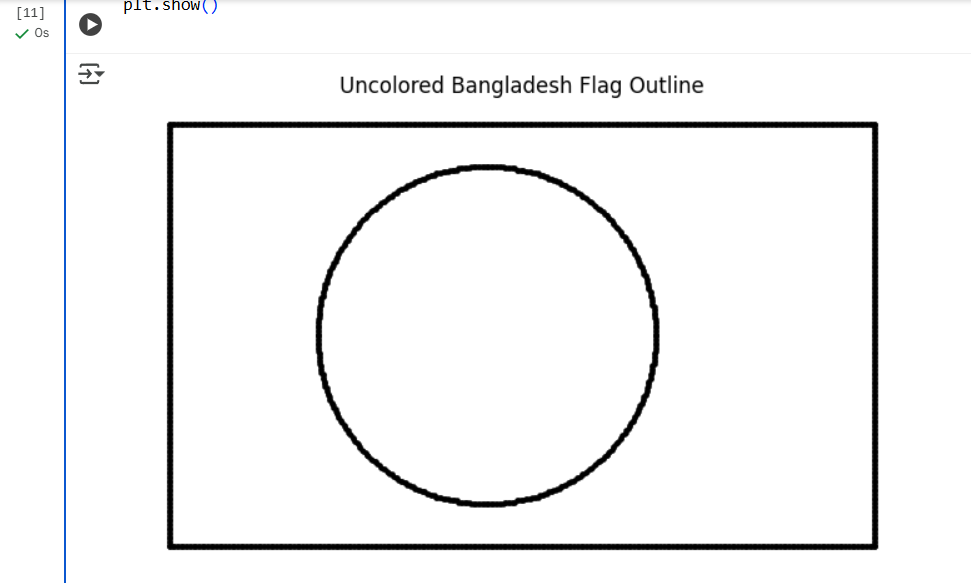
\includegraphics[width=1.0\textwidth]{uncolor.png}
    \caption{Shape of The Given Flag (Uncolored)}
\end{figure}

\begin{figure}[H]
    \centering
    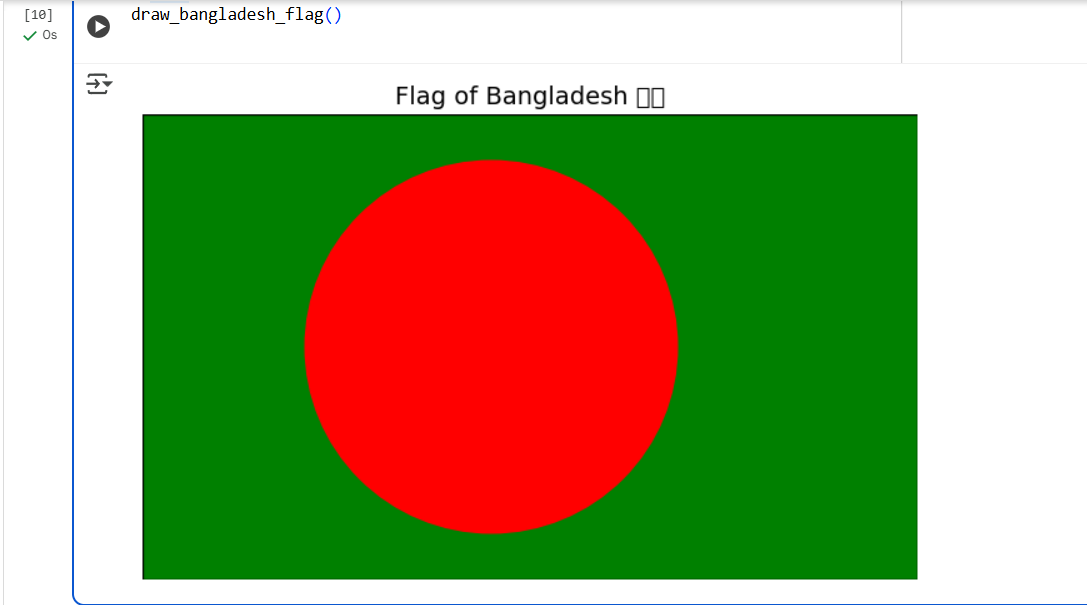
\includegraphics[width=1.0\textwidth]{bd_flag.png}
    \caption{Shape of The Given Flag (Colored)}
\end{figure}



\subsubsection*{Task 4: Reflection on Advantages and Limitations}
- \textbf{Advantages}: 
  - DDA provides high accuracy for line drawing with smooth interpolation.
  - Midpoint circle algorithm is efficient, requiring minimal computation for circle generation.
  - Flood fill ensures complete and uniform coloring of enclosed areas.
- \textbf{Limitations}: 
  - DDA can be computationally intensive due to floating-point operations.
  - Midpoint circle algorithm may introduce minor rounding errors.
  - Flood fill can be slow and memory-intensive for large areas due to recursive calls, potentially leading to stack overflow.

\subsection*{Complex Problem-Solving Questions}
\begin{enumerate}
    \item[a.] \textbf{Question: Does the solution need in-depth engineering knowledge?} \\
        \textbf{Answer: Yes, a deep understanding of graphics algorithms, including their mathematical underpinnings and practical implementation, is crucial for crafting an effective solution.}
    \item[b.] \textbf{Question: Does the solution involve wide-ranging or conflicting technical, engineering, or other issues?} \\
        \textbf{Answer: Generally, no major conflicts emerge, but optimizing the algorithms for varying screen resolutions and performance might pose a challenge that requires thoughtful adjustments.}
    \item[c.] \textbf{Question: Is the solution well-known, or does it require abstract thinking and analysis to formulate?} \\
        \textbf{Answer: The algorithms like DDA, Midpoint Circle, and Flood Fill are well-established in computer graphics, yet tailoring them to accommodate dynamic flag sizes demands analytical creativity.}
    \item[d.] \textbf{Question: Does the solution involve infrequently encountered issues?} \\
        \textbf{Answer: No, these are common graphics challenges frequently addressed in both academic and industry contexts.}
    \item[e.] \textbf{Question: Does the solution need adherence to standards and codes of practice?} \\
        \textbf{Answer: Yes, adherence to basic coding standards and graphics conventions, such as accurate color representation and pixel precision, is necessary.}
    \item[f.] \textbf{Question: Does the solution involve stakeholders with conflicting technical requirements?} \\
        \textbf{Answer: Not directly, though managing diverse client preferences for flag dimensions and color fidelity could present minor hurdles.}
    \item[g.] \textbf{Question: Does the solution involve interdependence between sub-problems or parts?} \\
        \textbf{Answer: Absolutely, the successful coloring of the flag relies on the precise completion of drawing the rectangle and circle beforehand.}
\end{enumerate}

\end{document}